%File: formatting-instruction.tex
\documentclass[letterpaper]{article}
\usepackage{aaai}
\usepackage{times}
\usepackage{helvet}
\usepackage{courier}
\usepackage{graphicx}
\frenchspacing
\setlength{\pdfpagewidth}{8.5in}
\setlength{\pdfpageheight}{11in}
\pdfinfo{
/Title (Insert Your Title Here)
/Author (Put All Your Authors Here, Separated by Commas)}
\setcounter{secnumdepth}{0}  
 \begin{document}
% The file aaai.sty is the style file for AAAI Press 
% proceedings, working notes, and technical reports.
%
\title{Trading Cryptocurrencies with\\Reinforcement Learning}
\author{University of Colorado Colorado Springs\\Jacob Quatkemeyer\\Caden Aragon
}
\maketitle
\begin{abstract}
\begin{quote}
Stock trading has taken place since the early 1800's. Stock trading is a complicated space to generate an income, however, those that excel at trading generate hefty incomes. A newer space in the world of trading is cryptocurrency. Much like traditional stocks, varying in price each second, traders buy and sell these coins in hope of making a profit. To accomplish such a goal, there are many trading strategies including: scalping, day trading, intraday trading. While many have been successful using these traditional trading techniques, this paper looks to explore reinforcement learning and deep reinforcement learning to optimize a cryptocurrency trading strategy that can outperform a human trader.
\end{quote}
\end{abstract}

\section{1 Introduction}
\noindent The first official cryptocurrency was Bitcoin, established in 2009. Each coin started trading at as low as \$0.008 per coin. Just over a twelve years later, a single Bitcoin reached the price of \$64,863. Many early investors made millions of dollars, while other investors lost fortunes. The problem with trading and investing in cypto coins is that without proper knowledge, it is mostly a gamble. A possible solution to combat human limitations and learning curve is to train an agent to read market indicators and recognize patterns using reinforcement learning. Then agent will then be able to buy, sell, and hold coins to generate a profit.

Furthermore, vital to the prediction of cryptocurrency movement are market indicators. Some of the most popular indicators include the relative strength index (RSI), Bollinger bands, moving average convergence divergence (MACD). A successful trading bot will be able to read multiple indicators, recognizing patterns, thus predicting a market buy, sell, or hold. This resulting in a profit.

Another issue with trading coins as a human, is the frequency in which you can trade coins. A trader has to read different indicators and execute actions. A trader is limited to trading smaller amounts over a period of time. Computers, even without the use of reinforcement learning, read the indicators and trade dozens of coins in a small period of time. Using this method is known as high frequency trading (HFT). This technique of trading involves holding many positions at a time, and earning a very small profit on a large number of transactions, leading to a sizeable profit (Huang, Huan, Xu, Zheng, \& Zou, 2019).

Other papers have tried to use different reinforcement learning algorithms to trade coins frequently, but the majority of researchers train their agent with: many indicators on a single coins, or even no indicators at all. They also tend to test only one algorithm, and measure them against the algorithms used by other researchers. In this paper, we aim to find a good mix between valuable indicators, heavily traded coins, and different reinforcement learning algorithms. 

We will start with a simple Q learning algorithm, to see determine the limitations of this method. Then, move to a Deep Q algorithm using a neural networks. The goal is to train our agent well enough to outperform human traders on the cryptocurrency trading market, and to find limitations upon different algorithms.

\section{2 Background}
Reinforcement learning began making its debate in the late 1900's. The basis of this learning takes an agent that has the goal of mapping states to actions, yielding the greatest numerical reward. The agent does so by exploring states in a given episode. In states, an agent may receive immediate rewards or a singular end of episode reward. All rewards may be negative or positive. Over time, the agent the agent will learn to take actions that obtain most optimal reward. Today, this method is applied in Natural Language Processing (NLP), industry automation, and finance applications. Regarding finance, there are many ways in which this learning technique can be applied to cryptocurrencies. In this attempt we will be using standard Monte Carlo Q learning approach, and a Monte Carlo deep Q learning algorithm. To measure the effectiveness, we will be using the overall profit and Sharpe Ratio.

\subsection{2.1 Q-Learning}
This an off-policy TD control algorithm. For this policy, where the agent's goal to obtain the ideal state-action function defined by

$Q(S_{t}, A_{t}) $\leftarrow$ Q(S_{t}, A_{t})+ $\alpha$ [R_{t+1}+ $\gamma$ maxQ(S_{t+1, a}-Q(S_{t}, A_{t})$


in which the learning rate is defined as $\alpha$. The immediate reward plus the discount factor is defined as, [R_{t+1}+ $\gamma$ maxQ(S_{t+1, a}. The actual Q-value is defined as Q(S_{t}, A_{t}).
In the approach, each action is mapped to a table defined as a Q-table. This table initially holds a set of null or zero values. As the agent takes actions the state-action pair value is updated by the function defined above. For correctness, the values will be updated every time state-action pairs are visited. In time, the agent will determine an optimal state-action pair.

\subsection{2.2 Deep Q-Learning} 
Deep Q-Learning (DQN) (Mnih et al., 2015) is a built from of the Q-Learning algorithm with three main contributions: a deep conventional neural net architecture for Q-function approximation,
the use of mini-batches of random training data rather than single-step updates on the last experience, and the use of older network parameters to estimate the Q-values of the next state. (Roderick, MacGlashan, \& Tellex, 2017). These contributions will allow us to provide the agent with more indicators and more training data without compromising the efficiency of the training. This will allow the agent to learn more about which action to perform, leading to a better policy.

\section{3 Related Work}
In 2001, Jae Won Lee, used a reinforcement learning approach to stock price prediction. Although this paper is from 2001, many modern papers are still citing it today because of its usefulness in the field (Shi, Li, Zh\&, Cambria, 2021). To accomplish this task, a Makarov approach was used, which in this case determines the optimal policy to be a prediction because every trader may make the claim to have an optimal strategy different from one another. Given this policy, the agent will make an action that will result in the highest cumulative reward. This follows the traditional approach to a Makarov process in which there is a state and reward, both likely unknown to the agent. In this case, the state is represented by a vector allocating the common values available to a trader on any given day. The reward is yielded using a combination of the immediate reward and closing price of the stock in each state space. Additionally, due to the continuously changing state space of a stock, a generalizing method is required since it is likely the state has never been experienced by the agent before. Using a nonlinear gradient based approximation, the agent can handle the ever-changing state space. This work proved to have some success in predicting the stock price.

\section{4 Methodology}
We will begin by training the agent on historical cryptocurrency trading data from multiple different coins using a Q learning algorithm. Training the data on different coins will avoid generalization, and will give the agent a greater range of data to learn from. Each time step of the data will be measured by the hour to take advantage of the 24 hour market that cryptocurrencies are sold on. The market is volatile enough to still make a profit using one hour time steps. We will then test the agent on a different range of data, to find out how profitable and reliable the Q-learning trained agent is for automated trading. The next step is to train a new agent using a Deep Q learning algorithm. This will take advantage of a multi-layered neural network. The agent in the same fashion. Given the efficiency of this new algorithm, it will be given more data to train on.

\subsection{4.1 Data}
To gather the data, we will be using an API from Binance, a crypto exchange. This will allow us to download any range of data from any coin on the market. It is a useful tool that we could implement into the training network, allowing the training program to dynamically download more data to learn from based on different parameters. The data can also be downloaded in a range of time steps such as 5 minutes, 15 minutes, 30 minutes, 1 hour, etc. We will begin by downloading data in 1 hour time steps.

\subsection{4.2 Training}
We will be training the agents using basic reinforcement learning concepts. We first define the state space. A state is given as the time step including the trading indicators. The amount of indicators will depend on the efficiency of the trading algorithm. A larger amount of indicators will provide a larger Q-Table, requiring more processing power (or a more efficient processing algorithm). In general, the most commonly used indicators in trading that can effectively be handled will be used. The action space is defined very simply, with only three actions: buy, sell, and hold. The agent will be rewarded positively for the amount of profit at the end of each day. The more profit, the more reward. The agent will be rewarded negatively for each loss. Again, the greater the loss, the greater the punishment.

\section{5 Evaluation}
The two agents will be evaluated with two values, overall profit and the Sharpe ratio. The Sharpe ratio is defined:
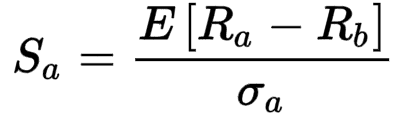
\includegraphics{Sharpe} 
\\
\\
where
\[ R_a = asset\ return \] 
\[ R_b = risk\ free\ return \] 
\[ E = expected\  value \] 
\[ \sigma_a = standard\ deviation\ of\ the\ asset\ excess\ return \] 

The Sharpe ratio defines the expected profit when accounting for loss. A portfolio can earn 100\% profit one month and obtain the image as an incredibly profitable strategy. However, if it loses 100\% for the next six months, then the trading strategy, or in our case the agents policy, is not efficient. The agent happened to get lucky during the first month. Profit is important, but only if the risk is also calculated. We will evaluate the Sharpe ratio that each agent is capable of earning to ensure that the agent profits without risking too much of of the overall assets.
	
\section{6 Timeline}
\begin{center}
\begin{tabular}{||c|c|||} 
 \hline
 Date & Task \\ [0.5ex] 
 \hline\hline
 09/29/2021 & Data Collected and Organized \\ 
 \hline
 10/06/2021 & Envrionment Created \\
 \hline
 10/13/2021 & Q-Learning Training Completed \\
 \hline
 10/16/2021 & Results Evaluated \\
 \hline
 10/18/2021 & Midterm Presentations \\ [1ex] 
 \hline
\end{tabular}
\end{center}

\section{7 Conclusion}
By starting out with a traditional Q-learning method, and graduating to a Deep Q Network learning method, we will investigate how neural networks can defeat many of the limitations seen by the earlier reinforcement learning methods. Furthermore, we are confident that the DQN learning method will produce a policy that produces more success than a human controlled portfolio trading under the same circumstances. Lastly, we also plan on finding a less generalized policy compared to the policies learned by agents in other research. The methodology of training on various coin's aims to resolve this. 

\section{References}
\smallskip \noindent \textit{B. Huang, Y. Huan}\\
Automated trading systems statistical and machine learning methods and hardware implementation: A survey Enterprise Information Systems, L.D. Xu, L. Zheng, Z. Zou 2019. \textit{Blackboard Systems.} 13 (1) (2019), pp. 132-144

\smallskip \noindent \textit{Roderick, M., MacGlashan, J, Tellex, S} 
Implementing the deep Q-network.  Humans To Robots Laboratory, Brown University, Providence, RI 02912, CoRR (2017)

\smallskip \noindent \textit{Mnih, V., Kavukcuoglu, K., Silver, D. et al}\\
Human-level control through deep reinforcement learning. Nature 518, 529–533 (2015). 
https://doi.org/10.1038/nature14236

\smallskip \noindent \textit{Jae Won Lee} 
Stock price prediction using reinforcement learning. ISIE 2001. 2001 IEEE International Symposium on Industrial Electronics Proceedings (Cat. No.01TH8570), 2001, pp. 690-695 vol.1, 
doi: 10.1109/ISIE.2001.931880.

\smallskip \noindent \textit{Yong Shi, Wei Li, Luyao Zhu, Kun Guo, Erik Cambria}
Stock trading rule discovery with double deep Q-network. Applied Soft Computing. Volume 107. 2021. 107320. ISSN 1568-4946.
https://doi.org/10.1016/j.asoc.2021.107320.


\end{document}
